%\chapter{Построение решения задачи}
\chapter{Построение решения задачи генерации UML-моделей по PDDL-описаниям}
   
%\section{Разметка моделей при помощи профиля планирования}
\begin{figure}[h]
    \centering
    \begin{minipage}{0.8\linewidth}
        \centering
        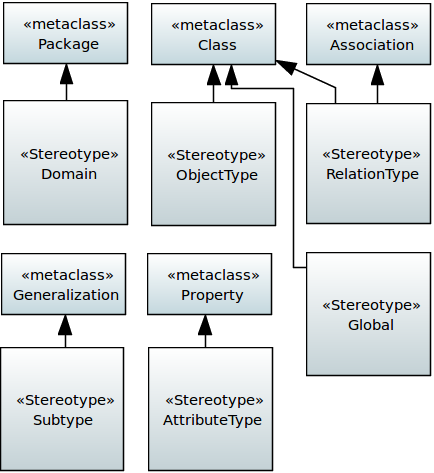
\includegraphics[width=0.8\linewidth]{stereo-domain}
        \caption{Диаграмма профиля со стереотипами для описания предметной области}
        \label{img:stereo-domain}
    \end{minipage}
\end{figure}

\begin{figure}[h]
    \centering
    \begin{minipage}{0.8\linewidth}
        \centering
        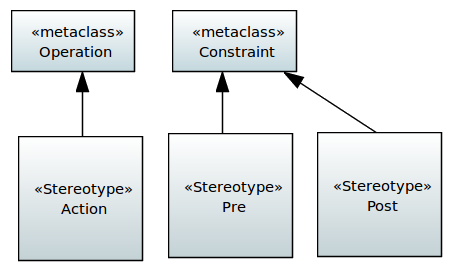
\includegraphics[width=0.8\linewidth]{stereo-actions}
        \caption{Диаграмма профиля со стереотипами для описания действий}
        \label{img:stereo-actions}
    \end{minipage}
\end{figure}

\begin{figure}[h]
    \centering
    \begin{minipage}{0.75\linewidth}
        \centering
        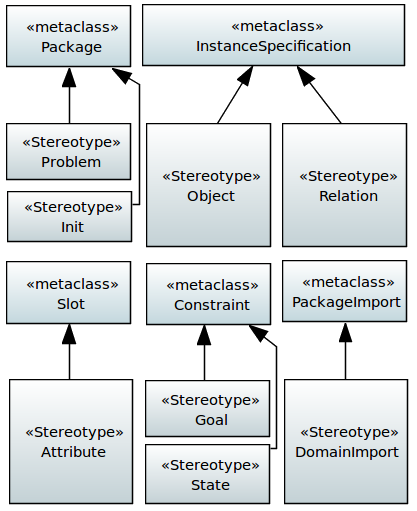
\includegraphics[width=0.8\linewidth]{stereo-states}
        \caption{Диаграмма профиля со стереотипами для описания задач и состояний}
        \label{img:stereo-states}
    \end{minipage}
\end{figure} 

В рамках работы \cite{mal-manz}  был предложено расширение UML для области планирования. В UML расширение осуществляется за счет расширения его метамодели посредством механизма профилей. Применение профиля планирования позволит нам использовать стереотипы, определенные в профиле. Таким образом, мы адаптируем UML для работы с новыми понятиями области планирования. 

С помощью применения стереотипов можно добиться уточнения семантики элементов, наделения элементов новыми свойствами. В нашем случае это может быть полезно, так как существуют средства, работающие с UML-моделями предметных областей и задач планирования, размеченными данными стереотипами. Таким образом можно добиться более тесной интеграции разрабатываемого инструмента с другими инструментами инженерии знаний.

В работе мы оперируем такими понятиями, как предметная область, которая будет размещена в UML-пакете (\texttt{package}), размеченном стереотипом  \stype{Domain}. В этом пакете будут находится классы со стереотипом \stype{ObjectType} и ассоциации со стереотипом \stype{RelationType}. Связи обобщения помечаются стереотипом \stype{Subtype}. Атрибуты классов будут иметь стереотип \stype{AttributeType} (рис.~\ref{img:stereo-domain}). Если для моделирования предметной области нужно задавать параметры среды, то в корне создается некий абстрактный класс, который помечается стереотипом \stype{Global}.


\iffalse
\begin{figure}[h]
    \centering
    \begin{minipage}{0.75\linewidth}
        \centering
        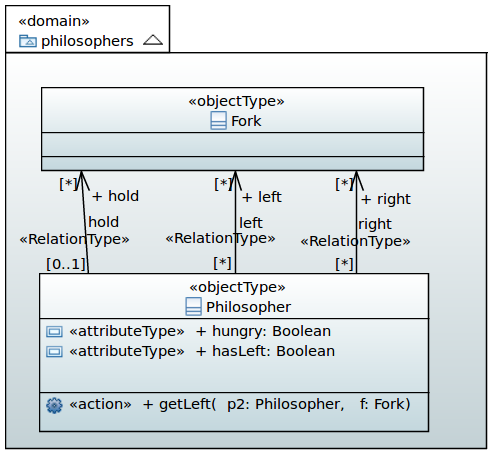
\includegraphics[width=0.8\linewidth]{stereo-domain-example}
        \caption{Диаграмма классов, размеченных стереотипами, для описания предметной области}
        \label{img:stereo-domain-example}
    \end{minipage}
\end{figure} 

\begin{figure}[h]
    \centering
    \begin{minipage}{0.75\linewidth}
        \centering
        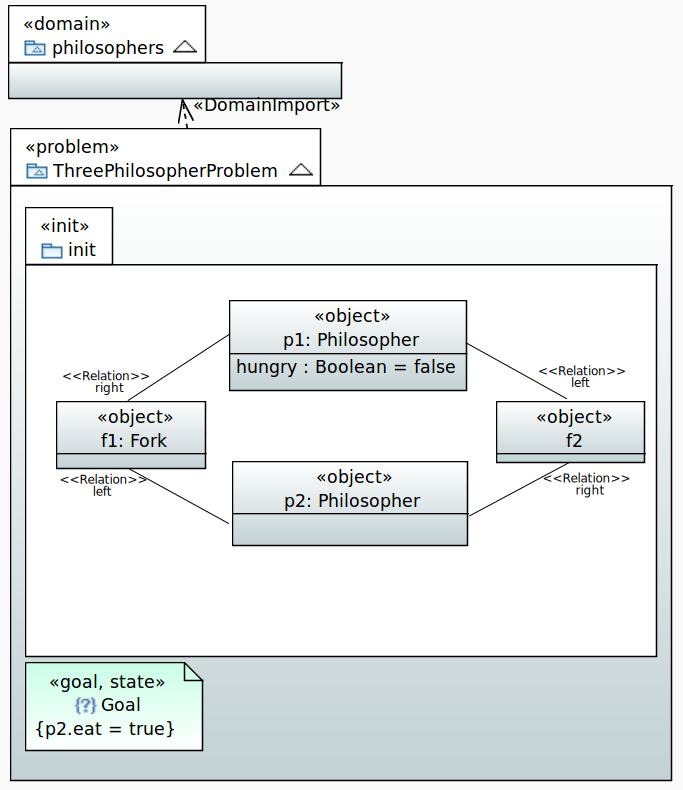
\includegraphics[width=0.8\linewidth]{stereo-problem-example}
        \caption{Диаграмма классов, размеченных стереотипами, для описания задач и состояний}
        \label{img:stereo-problem-example}
    \end{minipage}
\end{figure} 
\fi

Кроме того, метод класса должен быть размечен стереотипом \stype{Action}, а его пред- и пост-условия стереотипами \stype{Pre} и \stype{Post} соответственно (рис.~\ref{img:stereo-actions})

Задача планирования всегда находится в своем пакете, помеченном стереотипом \stype{Problem}. Если этот пакет будет находится в другой модели, отличной от модели предметной области, то от пакета задачи необходимо провести связь \texttt{PackageImport} к пакету предметной области, такая связь должна быть размечена стереотипом \stype{DomainImport}. Объекты (экземпляры класса) и связи (экземпляры ассоциации) представляются в UML с помощью экземпляров \texttt{InstanceSpecifications}, они должны быть размечены стереотипами \stype{Object} и \stype{Relation} соответственно. Экземпляры атрибутов помещаются в слоты объектов, они помечаются стереотипом \stype{Attribute}. Внутрь пакета с описанием задачи кладется пакет с описанием начального состояния задачи, этот пакет размечается стереотипом \stype{Init}. И, наконец, ограничения на состояния размечаются стереотипом \stype{State}, причем ограничение на конечное состояния должно размечаться дополнительно стереотипом \stype{Goal} (рис.~\ref{img:stereo-states}).

\iffalse
Разметка предметной области и задачи на примере фрагмента ПО ``Обедающие философы'' приведена на рисунках~\ref{img:stereo-domain-example}~и~\ref{img:stereo-problem-example}.

Готовых средств, решающих задачу, поставленную в данной дипломной работе, нет, поэтому оправдано создание собственного средства.

За основу разрабатываемой нотации на основе UML было решено взять нотацию, предложенную в статье \cite{mal-manz}, и, если необходимо, дополнить её новыми элементами UML или предложить новый способ представления элементов PDDL.
Данная нотация задает отображение UML-модели, размеченной стереотипами области планирования, в элементы PDDL. 
Это отображение использует не все возможности PDDL, поэтому для некоторых элементов PDDL обратное отображение пока не определено. 
Кроме того, для некоторых элементов, для которых ясно, как их представлять в UML, может быть не все так просто в связи с недостатком информации о предметной области.
\fi
Теперь исследуем преобразование PDDL-элементов в элементы UML и соответствие этого преобразования требованиям, представленным к работе.

%%%%%%%%%%%%%%%%%%%%%%%%%%%%%%%%%%%%%%%%%%%%%%%%%%%%%%%%%%%%%%

\section{Правила преобразования основных конструкций PDDL в элементы UML-модели}
%Разберем подробнее, как транслируются различные части PDDL описаний и с какими трудностями можно при этом столкнуться.

\subsection{Правила, относящиеся к описаниям предметной области}
    
В самом начале любого описания предметной области на PDDL находится название предметной области.
Оно преобразуется в UML-модель с соответствующим именем, как показано на рис. \ref{img:tr-domain} 

\translation{
\begin{alltt}
(define (domain philosophers)
   ...
)
\end{alltt}
}
{0.7}
{tr-domain}
{Пример преобразования начала описания предметной области}
{img:tr-domain}


\translation{
\begin{alltt}
...
(:types 
   A - object
   B - A
)
...
\end{alltt}
}
{0.4}
{tr-types}
{Пример преобразования классов}
{img:tr-types}

Каждый PDDL-тип преобразуется в UML-класс, как показано на рисунке \ref{img:tr-types}. При этом выполняется требование (\ref{eq:types}) для преобразования типов.

%%%%%%%%%%%%%%%%%%%%%%%%%%%%
%%%%%%%%%%%%%%%%%%%%%%%%%%%% Предикатики
Преобразование предикатов зависит от количества аргументов.

Если аргументов нет~--- предикат преобразуется в статический булев атрибут некоторого абстрактного класса, не имеющего прямого отношения к классам предметной области.  Этот класс содержит параметры среды.

Если аргумент один: $\langle arg_0 \rangle$~--- предикат преобразуется в булев атрибут класса, соответствующего типу $Type(arg_0)$.

Если аргументов несколько: $\langle arg_0, \ldots arg_n \rangle$~--- предикат преобразуется в ассоциацию. 
Ассоциация будет бинарной, если аргументов два, и n-арной, если аргументов больше, чем два. 
К сожалению, PDDL-описание не содержит в явном виде достаточно информации для восстановления кратностей концов ассоциации: без предположений о связях между объектами мы не можем ограничивать мощность ассоциации и обязаны преобразовать предикат в ассоциацию с концами максимальной мощности \texttt{[*]} (рис.~\ref{img:tr-assoc-m-m}). 

\translation{
\begin{alltt}
...
  (:predicates
    (pred1)
    (pred2 ?arg0 - A)
    (pred3 ?arg0 - A ?arg1 - B)
    (pred4 ?arg0 - A ?arg1 - B 
                     ?arg2 - C)
  )
...
\end{alltt}
}
{1}
{tr-assoc-m-m}
{Пример преобразования предикатов}
{img:tr-assoc-m-m}

С точки зрения инструментов, которые будут работать с конечной моделью в автоматическом режиме, данный нюанс не должен представлять каких-либо проблем.
Как мы увидим далее, получаемые формулы на языке OCL для ассоциаций с максимальными мощностями \texttt{[*]} выглядят очень громоздко, и, вероятно, пользователю-человеку будет довольно сложно разобраться в них и модифицировать при желании. 
Если бы удалось на одном из концов ассоциации установить мощность ``не более, чем один'' \texttt{[0..1]}, то это значительно сократило бы трудоёмкость получаемых формул и увеличило бы их читаемость. Эта задача рассматривается в следующей секции.

Преобразование предикатов отображает унарные предикаты в атрибуты, а дву- и более арные~--- в ассоциации, причем ассоциации отличны друг от друга, поэтому выполнено свойство (\ref{eq:predicates}).

%%%%%%%%%%%%%%%%%%%%%%%%%%%%%%%%%%%%%%%%%%%%%%%%%%%%%%
%%%%%%%%%%%%%%%%%%%%%%%%%%%%%%%%%%%% Действия

Кроме предикатов в PDDL для упрощения выражений и придания большей ясности описаниям активно используются флюенты~--- функции, возвращающие нечто на выходе (число если флюента числовая, объект~--- если объектная), причем возвращаемые значения могут отличаться в зависимости от состояния задачи. Стоит отметить, что флюенты не вычисляются при обращении, а просто возвращают то, что им было сказано возвращать последним. Для использования флюент в описании ПО должно быть указано требование \texttt{:fluents}.

Хотя формальные требования, которым должно удовлетворять преобразование флюент, не были представлены в данной работе, попытаемся рассмотреть и проанализировать это преобразование.

Флюенты  преобразуются в зависимости от количества аргументов, которые они принимают на вход:

Если аргументов нет~--- то это глобальная переменная (переменная среды), и её можно преобразовать в статический атрибут класса с параметрами среды. 

Если аргумент один: $\langle arg_0 \rangle$~--- флюенту можно преобразовать в атрибут класса-образа $Type(arg_0)$.

Если аргументов несколько (больше одного): $\langle arg_0, \ldots, arg_n \rangle$~--- то флюента преобразуется в атрибут класса-ассоциации, которая также создается между классами аргументов флюенты $\langle F_T(Type(arg_0), \ldots, F_T(Type(arg_n))) \rangle$, причем кратности концов этой ассоциации равны \texttt{[1]}. Т.е. каждому кортежу (упорядоченной последовательности) из $n+1$ объектов указанных типов ставится в соответствие класс ассоциации.
Сказанное выше показано на рисунке \ref{img:tr-fluents}. 

\translation{
\begin{alltt}
(:types A - object)
(:functions
  (attr1) - A
  (attr2 ?arg0 - A) - number
  (dist  ?arg0 - A 
         ?arg1 - A) - number
)
\end{alltt}
}
{0.7}
{tr-fluents}
{Пример преобразования флюент}
{img:tr-fluents}

Как видно из определения преобразования, разные флюенты PDDL преобразуются в разные элементы UML и элементы, которые получаются в результате преобразования флюент не будут конфликтовать с элементами, получающимися в итоге других преобразований (просто используются разные элементы). Поэтому такое преобразование флюент корректно относительно свойств, аналогичных свойствам преобразования предикатов.
\\

Рассмотрим, как преобразуются PDDL-действия.
Каждое действие состоит из описания параметров, предусловия и эффекта.

Образом каждого действия становится метод класса, к которому относится первый аргумент этого действия. При этом остальные аргументы записываются как параметры этого метода. Таким образом, действие без параметров отображается в статический метод абстрактного класса-среды. 

Согласно стандарту UML к операции можно прикреплять пред- и постусловия, представленные ограничениями (\texttt{Constraint}). 
Эффекты действий будут преобразовываться в постусловия. Значением ограничения в данном случае будет спецификация типа \texttt{LiteralString}, содержащая соответствующее OCL-выражение. На диаграмме классов это может быть изображено в качестве узла-ограничения.

Сказанное выше показано на рисунке \ref{img:tr-actions}. $OCL(expr)$ означает соответствующую PDDL-выражению expr формулу на языке OCL.

\translation{
\begin{alltt}
...
  (:action act1
    :parameters ()
    ...
  )
  (:action act2
    :parameters (?p1 - A ?p2 - B)
    :precondition expr1
    :effect expr2
  )
...
\end{alltt}
}
{0.7}
{tr-actions}
{Пример преобразования действий}
{img:tr-actions}

%%% Преобразование предусловия
Исходя из определенного преобразования действий, можно заключить, что выполняется свойство (\ref{eq:action}): все образы действий различны, семантика сохраняется.

Предусловия и эффекты действий описываются с помощью PDDL-выражений.
В UML моделировании принято записывать ограничения на языке OCL\footnote{OCL~--- Object Constraint Language}~--- языке объектных ограничений. Более детально трансляция выражений будет рассмотрена ниже.

%%%%%%%%%%%%%%%%%%%%%%%%%%%%%%%%%%%% Задачки 
%%%%%%%%%%%%%%%%%%%%%%%%%%%%%%%%%%%%%%%%%%%%%%%%%%%%%%%%%%%%%%%%%%%%%%%%
%%%%%%%%%%%%%%%%%%%%%%%%%%%%%%%%%%%%%%%%%%%%%%%%%%%%%%%%%%%%%%%%%%%%%%%%
%%%%%%%%%%%%%%%%%%%%%%%%%%%%%%%%%%%%%%%%%%%%%%%%%%%%%%%%%%%%%%%%%%%%%%%%
%%%%%%%%%%%%%%%%%%%%%%%%%%%%%%%%%%%%%%%%%%%%%%%%%%%%%%%%%%%%%%%%%%%%%%%%
%%%%%%%%%%%%%%%%%%%%%%%%%%%%%%%%%%%%%%%%%%%%%%%%%%%%%%%%%%%%%%%%%%%%%%%%
\subsection{Правила, относящиеся к описаниям задачи планирования}

Рассмотрим теперь как преобразуются описания задач.
У задачи есть название и указание на предметную область, к которой она относится. 
На каждую задачу выделяется отдельная UML-модель с соответствующим названием.
Указание на предметную область, к которой относится задача, преобразуется в связь типа \texttt{PackageImport} между моделями (рис.~\ref{img:tr-domain-import}).

\translation{
\begin{alltt}
(define 
    (problem ThreePhilosopherProblem)
    (:domain philosophers)    
    
    ...
)
\end{alltt}
}
{0.7}
{tr-domain-import}
{Трансляция заголовка задачи}
{img:tr-domain-import}

Затем, в описании перечисляются объекты, которые участвуют в задаче:

\begin{mdframed}[style=excode]
\begin{alltt}
  ...
  (:objects
      p1 - Philosopher
      p2 - Philosopher
      p3 - Philosopher
      f1 - Fork
      f2 - Fork
      f3 - Fork
  )
  ...
\end{alltt}
\end{mdframed}

Это описание не несет большой информационной нагрузки, его можно преобразовывать, а можно не преобразовывать. 
Так как в модель позднее будет помещено ограничение на конечное состояние, в котором будут использоваться эти объекты, то, чтобы было понятно, о каких объектах идет речь, это перечисление можно преобразовывать в экземпляры классов (\texttt{InstanceSpecification}), например, в корне модели задачи.

Задача в простом случае представляется как $T = \langle I, G \rangle$, где $I$~--- начальное состояние, представленное как набор фактов (положительных), не перечисленные факты считаются ложными; $G$~--- логическая формула, вычисляющаяся на состояниях, $G(s) = True \Leftrightarrow s$~--- целевое состояние. 
Описание начального состояния преобразуется так, как показано на рис.~\ref{img:tr-init}.


\translation{
\begin{alltt}
  ...
  (:init
    (= (flue a1) b1)
    (pred1 a1 b2)
    (pred2 a2)
    ...
  )
  ...
\end{alltt}
}
{0.9}
{tr-init}
{Пример преобразования начального состояния задачи}
{img:tr-init}

Это описание преобразуется в пакет с именем \texttt{Init} в модели задачи.
В этом пакете создаются экземпляры классов, участвующих в описании начального состояния, и экземпляры ассоциаций, затем к ним крепятся слоты (\texttt{Slot}), в которые помещаются значения (\texttt{Value}), представляющие собой 
спецификацию нужного типа: \texttt{LiteralInteger} в случае числовой флюенты, \texttt{InstanceValue} в случае объектной флюенты и для экземпляров ассоциаций, \texttt{LiteralBoolean} в случае унарного предиката.

Ограничение на конечное состояние $G$, представляющее собой логическое PDDL-выражение, преобразуется в UML-ограничение  (\texttt{Constraint}, содержащее выраженное строкой OCL-выражение.
%В корень модели помещается UML-ограничение), значением которого устанавливается спецификация типа \texttt{LiteralString}, содержащая соответствующее выражение на языке OCL. 
Пример применения преобразования цели показан на рис.\ref{img:tr-goal}.
\translation{
\begin{alltt}
  ...
  (:goal
    expr
  )
  ...
\end{alltt}
}
{0.5}
{tr-goal}
{Пример применения преобразования цели задачи}
{img:tr-goal}

Исходя из определенного выше преобразования задач, можно заключить, что выполняется свойство корректности(\ref{eq:task}): каждому целевому PDDL-состоянию соответствует целевое UML-состояние и обратно.

Если все предыдущие свойства выполняются, то можно заключить, что
выполняется и свойство корректности для планов (\ref{eq:plan}).

%%%%%%%%%%%%%%%%%%%%%%%%%%%%%%%%%%%%%%%%%%%%%%%%%%%%%%%%%%%%%%%%%%%%%%%%
%%%%%%%%%%%%%%%%%%%%%%%%%%%%%%%%%%%%%%%%%%%%%%%%%%%%%%%%%%%%%%%%%%%%%%%%
%%%%%%%%%%%%%%%%%%%%%%%%%%%%%%%%%%%%%%%%%%%%%%%%%%%%%%%%%%%%%%%%%%%%%%%%
%%%%%%%%%%%%%%%%%%%%%%%%%%%%%%%%%%%%%%%%%%%%%%%%%%%%%%%%%%%%%%%%%%%%%%%%
%%%%%%%%%%%%%%%%%%%%%%%%%%%%%%%%%%%%%%%%%%%%%%%%%%%%%%%%%%%%%%%%%%%%%%%%
\subsection{Соответствие между PDDL-выражениями и ограничениями OCL}

Основные выражения PDDL можно транслировать согласно следующей таблице:

{
    \renewcommand{\arraystretch}{1.3}
    \centering
    \ttfamily
    \begin{tabular}{|p{0.40\linewidth}|p{0.50\linewidth}|}
        \hline
        \normalfont\bfseries PDDL\:-выражение & \normalfont\bfseries OCL\:-выражение \\
        \hline
        (and expr1 ... exprN) & expr1 and expr2 and ... and exprN \\
        \hline
        (or expr1 ... exprN) & expr1 or expr2 or ... or expr \\
        \hline
        (not expr1) & not expr1\normalfont, если \texttt{expr1}~-- не атом и не выражение ``='' \\ 
        \hline
        (= expr1 expr2) & expr1 = expr2 \\ \hline
        (not (= expr1 expr2)) & expr1 <> expr2 \\
        \hline 
        (<comp> expr1 expr2) & expr1 <comp> expr2 \\
        {\small <comp>::= > | < | = | >= | <=} & \\
        \hline
        (<op> expr1 ... exprN) & expr1 <op> ... <op> exprN \\
        {\small <op>::= + | *} & \\
        \hline
        (- expr) & -expr \\ 
        \hline
        (pred)\normalfont, pred~-- предикат & GlobalEnvironment.pred = true \\ \hline
        (not (pred)) & GlobalEnvironment.pred = false \\ \hline
        (pred p1) & p1.pred = true \\ \hline
        (not (pred p1)) & p1.pred = false \\
        \hline
        (flue)\normalfont, flue~-- флюента& GlobalEnvironment.flue \\ \hline
        (flue p1) & p1.flue \\
        \hline
    \end{tabular}
}
\\[5pt]

%%%% Флюенты логические

Трансляция n-арных ($n \geq 2$) флюент и предикатов имеет несколько особенностей. Рассмотрим подробнее, как транслируются выражения с флюентами.

Как мы помним (рис.~\ref{img:tr-fluents}), бинарные и более флюенты транслируются в ассоциацию со связанным с ней классом ассоциации, содержащим один атрибут.

Предположим, что у нас есть бинарная флюента, например:
\begin{mdframed}[style=excode]
\begin{alltt}
  ...
  (:functions
    (dist ?from - A ?to - B) - number
  )
  ...
\end{alltt}
\end{mdframed}

Выражение с такой флюентой \texttt{(dist arg1 arg2)} транслируется в:
\begin{alltt}
arg1.dist->any(x | x.to = arg2).value
\end{alltt}

Ассоциация может быть рекурсивной для такой флюенты:
\begin{mdframed}[style=excode]
\begin{alltt}
  ...
  (:functions
    (dist ?from - A ?to - A) - number
  )
  ...
\end{alltt}
\end{mdframed}

В этом случае необходимо явно указать направление навигации от объекта:
\begin{alltt}
arg1.dist[to]->any(x | x.to = arg2).value
\end{alltt}

Трансляция выражений, содержащих n-арные ($n \ge 2$) флюенты происходит аналогично. Пусть дана флюента следующего вида:
\begin{mdframed}[style=excode]
\begin{alltt}
  ...
  (:functions
    (flue ?argName1 - T1 
          ?argName2 - T2 ... 
          ?argNameN - TN) - number
  )
  ...
\end{alltt}
\end{mdframed}

Выражение \texttt{(flue arg1 ... argN)} транслируется так:

\begin{alltt}
arg1.flue->any(x | x.argName2 = arg2 and ... and
                   x.argNameN = argN).value
\end{alltt}

Если среди типов $T2 \ldots TN$ есть совпадающий с $T1 = Ti$, то навигация 
такого типа возможна только при помощи указания имени роли:

\begin{alltt}
arg1.flue[argi]->any(x | x.argName2 = arg2 and ... and
                         x.argNameN = argN).value
\end{alltt}

Этого достаточно, чтобы транслировать логические выражения с флюентами, хотя в случаях большой арности получающиеся формулы будут довольно сложными, и, возможно, не очень понятными, особенно если они содержат аргументы с одинаковыми типами.


%% Предикаты логические
Рассмотрим теперь, как могут транслироваться логические выражения с бинарными предикатами. Допустим, есть предикат следующего вида:

\begin{mdframed}[style=excode]
\begin{alltt}
  ...
  (:predicates
    (pred ?argName1 - T1 ?argName2 - T2)
  )
  ...
\end{alltt}
\end{mdframed}

Такой предикат транслируется в ассоциацию между двумя классами, как было показано на (рис.~\ref{img:tr-assoc-m-m}). 
Для него предиката логические выражения будут транслироваться согласно следующей таблице:
\\

{
    \renewcommand{\arraystretch}{1.3}
    \small
    \centering
    \ttfamily
    \begin{tabular}{|p{0.35\linewidth}|p{0.60\linewidth}|}
        \hline
        \normalfont\bfseries PDDL\:-выражение & \normalfont\bfseries OCL\:-выражение \\
        \hline
          (pred arg1 arg2) & arg1.argName2->includes(arg2) \\
        \hline
          (not (pred arg1 arg2)) & arg1.argName2->excludes(arg2)\\
        \hline
          (pred arg1 ... argN) 
          & 
          arg1.argName2->includes(arg2) and ...\newline
          \rule{2em}{0em} and arg1.argNameN->includes(argN) \\
        \hline
          (not (pred arg1 ... argN))
          &
          arg1.argName2->excludes(arg2) or ...\newline
          \rule{2em}{0em} or arg1.argNameN->excludes(argN) \\
        \hline

    \end{tabular}
}
\\[5pt]
%%% Преобразование эффекта

%%% флюенты эффекта
Эффект действия является не логическим выражением, которое должно вычисляться в $True$ для состояния, получающегося после применения действия, а является инструкцией по изменению конкретных фактов состояния. В связи с этим в эффектах можно встретить указания по изменению флюент. 

К сожалению, на OCL нельзя задать эффект действия, т.к. есть только возможность задать контракты действий: пару предусловие-постусловие. Постусловие аналогично предусловию: оно указывает, какому логическому выражению удовлетворяют состояния объектов после совершения действия. Для трансляции PDDL-эффекта в OCL-постусловие может потребоваться обращаться к значению флюент и предикатов в состоянии, предшествующем вызову метода. Для этого в языке OCL используется конструкция \texttt{@pre}. Трансляция основных выражений с флюентами показана в следующей таблице:
\\[2pt]

{
    \renewcommand{\arraystretch}{1.3}
    \small
    \centering
    \ttfamily
    \begin{tabular}{|p{0.35\linewidth}|p{0.60\linewidth}|}
        \hline
        \normalfont\bfseries PDDL\:-выражение & \normalfont\bfseries OCL\:-выражение \\
        \hline
        (<assign-op> (flue) expr)
                &
                GlobalEnvironment.flue = expr\normalfont,\newline
                \rule{1em}{0em}если \texttt{<assign-op> = assign;}\newline\ttfamily
                GlobalEnvironment.flue = \newline
                \rule{1em}{0em}GlobalEnvironment.flue@pre <op> expr\normalfont, иначе.
                \\ 
        \hline
                (<assign-op> \newline \rule{1em}{0em} (flue arg1) expr)
                & 
                arg1.flue = expr\normalfont, если \texttt{<assign-op> = assign};\newline \ttfamily 
                arg1.flue = arg1.flue@pre <op> expr\normalfont, иначе.
                \\
        \hline
            (assign \newline
            \rule{1em}{0em}(flue arg1) undefined) & arg1.flue = null \\
        \hline
            <assign-op>::= & <op>::= \\
             \raggedleft  assign & = \\
             \raggedleft  increase & + \\
             \raggedleft  decrease & - \\
             \raggedleft  scale-up & * \\ 
             \raggedleft  scale-down & / \\
        \hline
            (<assign-op> (flue\newline 
            \rule{2em}{0em}  arg1 ... argN) expr) 
            &
            arg1.flue->any(x | x.argName2 = arg2 and ... \newline
            \rule{1em}{0em} and x.argNameN = argN).value = expr\normalfont,\newline
            \rule{1em}{0em} если \texttt{<assign-op> = assign};\newline\ttfamily
            arg1.flue->any(x | x.argName2 = arg2 and \newline
            \rule{1em}{0em} ... and x.argNameN = argN).value = \newline
            arg1.flue@pre->any(x | x.argName2 = arg2 and \newline
            ... and x.argNameN = argN).value@pre<op> expr\normalfont,\newline
            \rule{1em}{0em} иначе. \\
        \hline
    \end{tabular}
}
\\[5pt]

%%%% Предикаты эффекта

Все, что было сказано о предикатах ранее~--- относилось к предикатам, встречающимся в логических выражениях, т.е. в предусловиях действий и в описаниях начальных состояний задач. Трансляция предикатов, находящихся в эффектах действий сталкивается с некоторыми проблемами помимо тех, которые обсуждались применительно к флюентам.

Согласно синтаксису языка PDDL, эффект действия описывается как конъюнкция положительных и отрицательных фактов о предикатах, а также фактов о флюентах. Последние мы обсуждали ранее.
Трансляция нуль- и ун-арных предикатов в эффектах уже была рассмотрена. 

Взглянем подробнее на n-арные ($n \geq 2$) предикаты. Описание эффекта, касающееся данных предикатов, можно разделить на две части $\langle Effect = Effect^-, Effect^+ \rangle$, где $Effect^-$~-- факты, которые должны быть удалены (или, по-другому, станут ложными в результирующем состоянии), и $Effect^+$~-- факты, которые должны быть добавлены (или, станут истинными в результирующем состоянии). Так как образами этих предикатов являются ассоциации, экземпляры которых логически соединяют множества объектов (в общем случае), то при трансляции нужно накладывать ограничение на изменение только тех объектов множества, которые затрагиваются этим действием, и никаких других. На помощь помимо уже знакомой конструкции \texttt{@pre} приходит операции добавления и удаления из множества \texttt{including} и \texttt{excluding}. Если кратности концов ассоциации не ограничены сверху 1, то необходимо использовать эти операции над множествами.

Но в данном случае получается не все просто, например, для следующего фрагмента:

\begin{mdframed}[style=excode]
\begin{alltt}
  ...
  (:effect
    (and (pred arg1 arg2)
         (not (pred arg1 arg3))
    )
  )
  ...
\end{alltt}
\end{mdframed}

Если транслировать его ``в лоб'', то получится противоречивое утверждение:

\begin{alltt}
  arg1.pred = arg1.pred@pre->including(arg2) and
  arg1.pred = arg1.pred@pre->excluding(arg2)
\end{alltt}

Чтобы все работало корректно, необходимо разбить эффект на группы по первому объекту.
Пусть у действия есть набор переменных-объектов, которыми оно оперирует $arg_0, \ldots, arg_n$.
Атом (он же факт) $atom = \langle pred, arg_{i_0}, arg_{i_1}, \ldots arg_{i_l} \rangle$.
Определим множества $Effect^-(pred_i, arg_i) = \{ atom | atom \in Effect^-, pred = pred_i, arg_{i_0} = arg_i \}$ и 
$Effect^+_(arg_i) = \{ atom | atom \in Effect^+,  arg_{i_0} = arg_i \}$. Тогда преобразование предикатов PDDL-эффекта можно осуществить согласно приведенной таблице:
\\

{
    \renewcommand{\arraystretch}{1.3}
    \small
    \centering
    \begin{tabular}{|p{0.35\linewidth}|p{0.60\linewidth}|}
        \hline
        \normalfont \bfseries PDDL\:-выражение & \normalfont\bfseries OCL\:-выражение \\
        \hline
          (and (pred $arg_0$ $arg_1$) ... \newline 
          \rule{2em}{0em} (pred $arg_0$ $arg_n$) \newline
          \rule{2em}{0em} (not (pred $arg_0$ $arg_{n+1}$)) ... \newline
          \rule{2em}{0em} (not (pred $arg_0$ $arg_m$)) \newline 
          ) & 
          $arg_0$.pred = $arg_0$.pred@pre->excluding($arg_{n+1}$)->\newline
          \rule{2em}{0em} ...->excluding($arg_m$)->including($arg_1$)->\newline
          \rule{2em}{0em} ...->including($arg_n$)\\
        \hline
          (and (pred $arg_0$ $arg_1$ $arg_2$)\newline 
          \rule{2em}{0em} (not (pred $arg_0$ $arg_3$ $arg_4$))\newline
          ) &
          $arg_0$.argName1 = $arg_0$.argName1@pre->excluding($arg_3$) \newline
          \rule{2em}{0em} ->including($arg_1$) and \newline
          $arg_0$.argName2 = $arg_0$.argName2@pre->excluding($arg_4$) \newline
          \rule{2em}{0em} ->including($arg_2$) \\
        \hline

    \end{tabular}
}
\\[5pt]
%%% конец преобразования выражений в OCL
%Вернемся теперь к трансляции элементов PDDL.
%У действий есть предусловия и эффекты, они могут быть представлены на языке OCL. Действия транслируются в UML-операции (\texttt{Operation}). Согласно стандарту UML к операции можно прикреплять пред- и постусловия, представленные ограничениями (\texttt{Constraint}). Значением ограничения в данном случае будет спецификация типа \texttt{LiteralString}, содержащая соответствующее OCL-выражение. На диаграмме классов это может быть изображено в качестве узла-ограничения.

\section{Способы пополнения генерируемой модели сведениями, не заданными явно во входных описаниях}
%\label{ocl-translation}

Чтобы была возможность извлечь типы из описания предметной области, она должна содержать соответствующую информацию, и в секции требований (\texttt{:requirements}) должно быть указано \texttt{:typing}. 
Если информации о типах в описании нет, то высказывать какие-либо предположения о типах объектов и аргументов действий невозможно.
В этом случе, все они будут типа \texttt{object}, базового для PDDL и все они будут транслироваться в UML-класс \texttt{Object} (рис. \ref{img:tr-untyped}).

\translation{
\begin{alltt}
(:predicates
  (hungry ?phi)
  (hasLeft ?phi)
  (left ?phi ?fork)
  ...
)
(:action getLeft
  :parameters (?p1 ?p2 ?f)
  ...
) 
\end{alltt}
}
{0.7}
{tr-untyped}
{Трансляция в случае отсутствия информации о типах}
{img:tr-untyped}


Как уже говорилось ранее, транслированные PDDL-выражения с предикатами, которые преобразуются в ассоциации с неограниченными кратностями концов, выглядят громоздко и с ними сложно оперировать. Поэтому, имеет смысл определить кратности ассоциаций более точно.
В этом может помочь только новая информация: не представленная явно в описании предметной области и задач планирования, но неявно в ней присутствующая, или пришедшая извне, например, от пользователя.

Во многих предметных областях и задачах существуют неявные ограничения на мощности концов, которые связаны прежде всего с требованиями/изменениями унарных предикатов в действиях. 
Этим изменениям сопутствуют изменения бинарных предикатов. 
Таким образом, если при анализе действий удастся выявить действия (или пары действий), которые по унарному предикату в предусловии взаимно исключают друг друга и одновременно с этим изменяют один и тот же бинарный предикат, то можно с большой уверенностью предположить, что этот бинарный предикат имеет ограниченную мощность.

\translation{
\begin{alltt}
(:action getLeft
  :parameters 
    (?p1 - Philosopher 
     ?p2 - Philosopher ?f - Fork)

  :precondition 
    (and (left ?p1 ?f)
         (right ?p2 ?f) 
         \textit{(hungry ?p1)}
         \textit{(not (hold ?p2 ?f))}
    )
      
  :effect
    (and (hasLeft ?p1)
         \textit{(hold ?p1 ?f)}
         \textit{(not (hungry ?p1))}
    )
)
\end{alltt}
}
{0.7}
{tr-assoc-1-m}
{Восстановление кратности из описания действия \texttt{[0..1]}}
{img:tr-assoc-1-m}

Более формально это можно описать следующим образом.
Предположим, что действие $a = \langle Pre_a, Effect_a \rangle$ описано в типичном для STRIPS стиле, т.е.:
\begin{center}
$Pre_a = \langle Pre_a^-, Pre_a^+ \rangle = \neg Pre_a^- \cup Pre_a^+ $,\\
$Pre_a^-, Pre_a^+ \subset Atoms_a$, \\
$Effect_a = \langle Effect_a^-, Effect_a^+ \rangle = \neg Effect_a^- \cup Effect_a^+$, \\
$Effect_a^-, Effect_a^+ \subset Atoms_a$,\\
\end{center}
где $Atoms_a$~--- множество всех фактов обо всех объектах, доступных для использования в действии $a$. $Pre_a^-, Pre_a^+$ представляют собой ограничение на состояние: одни факты должны быть истины (присутствуют в состоянии), а другие~--- точно ложны (отсутствуют в состоянии), или, что тоже самое, истинны отрицания этих атомов.
Истинность фактов, которые не упоминаются, не имеет значения. 
$Effect_a^-, Effect_a^+$~--- это факты, которые удаляются и добавляются к состоянию после применения действия, соответственно.
Если $Pre_a^+ \cap Effect_a^- \not= \emptyset$ или $Pre_a^- \cap Effect_a^+ \not= \emptyset$, что эквивалентно $I = Pred_a \cap \neg Effect_a \not = \emptyset$ и при этом $I$ содержит факт об унарном предикате, то анализируем действие дальше. 
Надо рассмотреть факты о предикатах, которые затрагивают один и тот же объект, если такие факты существуют, то можно сделать предположение о кратностях противоположных концов. Рассмотрим сказанное выше на примере действия \texttt{getLeft} из предметной области ``Обедающие философы''(рис.~\ref{img:tr-assoc-1-m}).

У данного действия в предусловии проверяется предикат \texttt{hungry}, а в эффекте этот же предикат удаляется.
Посмотрим, какие изменения сопутствуют изменению этого предиката.
Одновременно с ним меняется предикат \texttt{hold} с неизменным вторым вторым аргументом \texttt{?f}. 
Можно предположить, что противоположный конец \texttt{philosopher} соответствующей ассоциации имеет кратность не более 1.

Кроме такого анализа действий можно предложить анализировать задачи для предметной области. 
Если набор задач будет достаточно хорошим, то на основании того, какие в задачах даются начальные условия, можно выдвинуть предположения о мощностях ассоциаций. 
\begin{wrapfigure}{r}{0.4\linewidth}
{\centering
    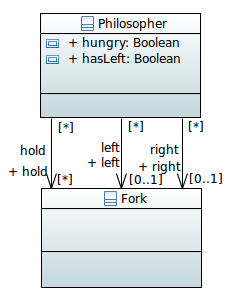
\includegraphics[width=\maxwidth{0.9\linewidth},keepaspectratio]{tr-assoc-m-1}
    \caption{Восстановление кратности из задачи планирования}\label{img:tr-assoc-m-1}
}
\end{wrapfigure}
В задаче, представленной на рис.~\ref{img:its-states}, для все той же предметной области видно, что каждый философ имеет не более одной вилки справа и не более одной вилки слева от него (на самом деле, в точности одну), поэтому можно предположить соответствующую кратность у ассоциаций \texttt{left} и \texttt{right}, как показано на рисунке \ref{img:tr-assoc-m-1}.

Разрабатываемый инструмент может предлагать пользователю в интерактивном режиме утверждать или отвергать данные предположения.
Если предположение утверждено~--- то учесть его при трансляции ассоциаций и выражений. 
Если предположение отвергнуто~--- то можно выдвинуть другое предположение (например, более слабое), а если предположений не осталось~--- оставить неограниченную мощность у ассоциации.

%%%%%%%%%%%%%%%%%%%%%%%%%%%%%%%%%%%%%%%%%%%%%%%%%%%%%%%%%%

%Если не удалось получить информацию о кратностях концов, то предполагается наиболее общий случай \texttt{[*]}. \tabularnewline



% Как правило, в предусловиях действий и в описаниях начальных состояний задач указывается большое количество утверждений об атомах (положительных или отрицательных), поэтому получившееся после трансляции OCL-выражение будет выглядеть довольно громоздким и плохо обозримым. Но с этим ничего нельзя поделать, если никак не удастся ограничить кратности концов ассоциации.

Предположим, что для бинарного предиката удалось каким-либо образом ограничить кратность второго конца ассоциации \texttt{argName2} хотя бы до \texttt{[0..1]}. Тогда основные логические выражения будут транслироваться несколько проще. Это отображено в таблице ниже:
\\

{
    \renewcommand{\arraystretch}{1.3}
    \small
    \centering
    \ttfamily
    \begin{tabular}{|p{0.35\linewidth}|p{0.60\linewidth}|}
        \hline
        \normalfont\bfseries PDDL\:-выражение & \normalfont\bfseries OCL\:-выражение \\
        \hline
          (pred arg1 arg2) & arg1.argName2 = arg2 \\
        \hline
          (not (pred arg1 arg2)) & arg1.argName2 <> arg2\\
        \hline
          (pred arg1 ... argN) 
          & 
          arg1.argName2 = arg2 and ...\newline
          \rule{2em}{0em} and arg1.argNameN = argN \\
        \hline
          (not (pred arg1 ... argN))
          &
          arg1.argName2 <> arg2 or ...\newline
          \rule{2em}{0em} or arg1.argNameN <> argN \\
        \hline

    \end{tabular}
}
\\[5pt]



%Итак, напомним, что PDDL-эффект описывает изменения объектов в результате применения действия в некотором состоянии. UML-постусловие действия задает логическое ограничение на состояние после применения действия. Для этого может использоваться конструкция OCL \texttt{@pre}.




\newpage